%\iffalse
%
%    \begin{macrocode}
%<*driver>
\documentclass{article}
\usepackage{doc}
\usepackage[american]{babel}
\usepackage[colorlinks,linktocpage=true]{hyperref}
\begin{document}
   \DocInput{ths.dtx}
\end{document}
%</driver>
%    \end{macrocode}
%\fi
%
% \title{Thesis/Dissertation Templates}
% \author{Kelly O.\ Homan, PhD\\
%         Associate Professor of Mechanical Engineering\\
%         Missouri University of Science \& Technology\\
%         Rolla, Missouri 65409-0050
%         \texttt{khoman@mst.edu}}
% \date{\LaTeX'd \today}
% \maketitle
%
% \begin{abstract}
% The templates contained in this \texttt{ltxdoc} file have been
% debugged with the 2018/08/07 version of \texttt{mstogs.cls}.
% \end{abstract}
%
% \tableofcontents
%
% \section{Preface}
% 
% \subsection{File Description}
%
% Simply \LaTeX\ the \verb|ths.ins| file to generate the template
% files for a publication thesis option format thesis,
% \verb|ptotemplate.tex|, and a \LaTeX-standard report class thesis,
% \verb|rpctemplate.tex|, along with five variants of a thesis
% chapter. The variants include text only (\verb|chapmin.tex|), floats
% (\verb|chapflt.tex|), bibliography citations (\verb|chapbib|),
% nomenclature entries (\verb|chapglo.tex|), and all of the above
% (\verb|chapall.tex|).  The inclusion or removal of these various
% chapter templates allows one to verify a local \LaTeX\ installation
% and the associated compile stages.
%
% This documentation file (\verb|ths.dtx|) can
% be typeset by running it through \LaTeX.
% 
% \emph{Very important:} the \verb|<ps>| characters which appear in
% the code are simply a placeholder for a percent sign (\LaTeX\
% comment character).  These characters are used so that during the
% generation of the code output, these lines are not removed.  Bottom
% line, after \LaTeX'ing the \verb|ths.ins| file, do a replace all for
% \verb|<ps>| with \verb|%| to obtain a proper \LaTeX\ file.
%
% \subsection{Limitations and Bugs}
% 
% \begin{description} 
% \item [Added: 2014/10/21] The documentation text may not accurately
% reflect the current form of the code.  The code, however, is correct
% and produces properly functioning templates.
% \item [Added: 2011/10/24] 
%  The co-adviser specification does not work as indicated by the 
%  original template.  The command must have an error in it as the
%    command desires an argument, but when one is provided, it adds
%    the designation co-adviser to the committee memberone.
% \item [Resolved (Originally Added: 2011/11/03).] The first page of
%   each individual appendix in a thesis with multiple appendices is
%   not correctly generated in LaTeX.  At the moment, this would
%   require generating these pages outside of LaTeX.  The associated
%   class file will need revision in order to make these pages
%   generate with the correct formatting.
% \item [Added: 2008/01/23, Resolved: 2011/07/12]
%  At present the rpctemplate.tex will not be a function template.
%  This can be developed later on an as needed basis.  The intended
%  difference between the two templates is that the \verb|ptotemplate|
%  is a thesis based on the publication option whereas the
%  \verb|rpctemplate| is a thesis based on the report class and not
%  based on separately generated publication- formatted
%  manuscripts. 
% \end{description}
%
% \section{Hints for Final Edit Stage}
%
% The last stages of editing a thesis often come down to treating
%    widow and orphan lines.  The following are hints for addressing
%    these final issues:
% \begin{itemize}
% \item Use \verb|\enlargethispage{\baselineskip}| command.
% \item Add a \verb|\newpage| command to force the start of a new page
%    at a specific point.
% \item LaTeX has a parameter for 'penalty' for widows and orphans 
%    ('club lines' in LaTeX terminology). With the greater penalty
%    LaTeX will try more to avoid widows and orphans. You can try to 
%    increase these penalties by putting following commands in your 
%    document preamble:
%    \verb|\widowpenalty=300\clubpenalty=300|. If this does not help,
%    you can try increasing these values even more, to a maximum of 
%    10000. However, it is not recommended to set this value too high, 
%    as setting it to 10000 forbids LaTeX from doing this altogether, 
%    which might result in strange behavior.
% \item Although I have not tested this, Wikipedia suggests it also 
%    helps to have rubber band values for the space between paragraphs:
%    \verb|\setlength{\parskip}{3ex plus 2ex minus 2ex}|.
% \end{itemize}
%
% \section{\LaTeX\ Template for Standard Report Class Thesis}
%
% \subsection{Description}

% This template represents a thesis generated as a single report class
% document.
%
% I have used the \texttt{chapter} and \texttt{chapter*} commands to
% produce both chapter titles and titles for the frontmatter and
% backmatter.  In my opinion this is the easiest and most transparent
% method to produce absolutely uniform type and layout.  The thesis
% style files that I received tried to accomplish this using custom
% defined commands but the result was not satisfactory, in my opinion.
% The \texttt{chapter*} command produces no numbering, which is in
% fact true for any of the sectioning commands.
%
% One change which you, as a user, may wish to make is in the relative
% locations of the files.  For \LaTeX\, all relative file locations
% have to be given with respect to the file that will be compiled by
% \LaTeX. Thus, if it is desired to have chapter files in
% sub-directories of the directory containing the base \verb|*.tex|
% file, the include commands will need to be of a form such as
% \verb|\include{subdir/foo.tex}|. This same logic also applies to the
% locations used to specify the *.eps files in each of the chapter's
% \texttt{*.tex} files.  
% 
% The contents of \texttt{template.tex} are expected to be rather
% transparent.  The only thing that may be worth further explanation
% is the use of the \texttt{include} and \texttt{includeonly} commands
% instead of \texttt{input}.  The reason is that the
% include/includeonly combination allows one to conditionally load the
% files.  This can save time when only one chapter, or portion of the
% thesis, is begin worked on at a given time. The only danger to this
% approach is that if a given chapter is not part of the include only
% list, then its impact on pagination, lists of figures, tables, etc
% will be frozen.  A final run with all of the include files part of
% of the includeonly list will ensure a complete document.
%
% \subsection{Thesis Template}
%
% \subsubsection{Preamble}
%
%    \begin{macrocode}
%<*rpc>
 % -*- mode: LaTeX -*-
 % ... preamble ...
\documentclass[times,12pt,titlepage]{mstogs}
\doublespacing
\usepackage[authoryear,sort]{natbib} % ... numbers or authoryear ...
\setlength{\bibhang}{0.5in}
\usepackage{threeparttable}
\usepackage[final]{graphicx}
\usepackage{psfrag}
\usepackage[noprefix]{nomencl}
\makenomenclature
 % ... nomenclature groupings ...
\renewcommand{\nomgroup}[1]{
   \ifthenelse{\equal{#1}{A}}{\medskip \item \textbf{Roman}}{}%
   \ifthenelse{\equal{#1}{G}}{\medskip \item \textbf{Greek}}{}%
   \ifthenelse{\equal{#1}{S}}{\medskip \item \textbf{Subscripts}}{}%
}
 % ... nomenclature preamble ...
\renewcommand{\nompreamble}{%
\hspace*{-0.50in}\makebox[1.0in][l]{Symbol} Description}
\renewcommand{\nomlabelwidth}{1.0in}

\usepackage[nopar]{lipsum} % ... provides dummy text ...

 % ... end preamble ...

\begin{document}

%    \end{macrocode}
%
% \subsubsection{Title Page}
%
%    \begin{macrocode}
 % ... specify: ms or phd ...

\begin{ThesisTitlePage}{phd}

 % ... title page info ...

\author{\MakeUppercase{Full Legal Name}}

\thesistitle{\MakeUppercase{The Title of My Work}}

\department{Mechanical Engineering} 

 % ... thesis committee ...

\ThesisAdvisor{Ludwig Prandtl, Co-Advisor\\ Joe Miner, Co-Advisor}

\ThesisCommittee{%
Daniel Bernoulli\\ %
Leonard Euler\\ %
Pierre-Simon Laplace\\ %
Joseph Fourier}

 % ... Graduation date - NOT your submission date ...
\graddate{1685}       

\end{ThesisTitlePage}
%    \end{macrocode}
%
% \subsubsection{Copyright, Abstract, and Acknowledgements}
%
%    \begin{macrocode}
 % ... copyright page - true|false ...

\copyrightyear{1685}   
\ThesisCopyrightPage{true}

 % ... front matter - thesis abstract ...

\begin{ThesisAbstract}
\lipsum[1]
\end{ThesisAbstract}

 % ... front matter - thesis acknowledgements ...

\begin{ThesisAcknowledgment}
\lipsum[2-3]
\end{ThesisAcknowledgment}
%    \end{macrocode}
%
% \subsubsection{Contents, Illustrations, Tables and Symbols}
%
%    \begin{macrocode}
\begin{ThesisFrontMatter}
\tableofcontents 
\listoffigures 
\listoftables  
\listofsymbols
\end{ThesisFrontMatter}
%    \end{macrocode}
%
% \subsubsection{Thesis Body}
%
%    \begin{macrocode}

\begin{ThesisBody}

 % ... introduction chapter ...
\ThesisBodyChapter{Introduction}\input{chpone}
 % ... chapter ...
\ThesisBodyChapter{Literature Review}\input{chptwo}
 % ... chapter ... 
\ThesisBodyChapter{First Contribution With a Long and Complicated Title But
  No Citations or Nomenclature}\input{chpthree}
 % ... chapter ...
\ThesisBodyChapter{Second Contribution}\input{chpfour}
 % ... conclusions chapter ...
\ThesisBodyChapter{Conclusions}%%
%% This is file `chpfive.tex',
%% generated with the docstrip utility.
%%
%% The original source files were:
%%
%% ths.dtx  (with options: `chapmin')
%% 
%% IMPORTANT NOTICE:
%% 
%% For the copyright see the source file.
%% 
%% Any modified versions of this file must be renamed
%% with new filenames distinct from chpfive.tex.
%% 
%% For distribution of the original source see the terms
%% for copying and modification in the file ths.dtx.
%% 
%% This generated file may be distributed as long as the
%% original source files, as listed above, are part of the
%% same distribution. (The sources need not necessarily be
%% in the same archive or directory.)


 %% ... sample chapter ...

\lipsum[6]

\section{A SECOND-LEVEL HEADING}
\lipsum[7-9]

\subsection{A Third-Level Heading}
\lipsum[10]
\subsubsection{A fourth-level heading with a very long and complicated title
to once again verify the formatting}
\lipsum[10-12]
\subsubsection{Another fourth-level heading}
\lipsum[10-12]

\subsection{Another Third-Level Heading but with a Very Long and
  Complicated Title to Verify the Formatting}
\lipsum[13-15]

\section{Discussion Using a Second-Level Heading
  Which is Really Long So That It Produces a Two-Line
  Toc Entry}
\lipsum[10-12]


\endinput
%%
%% End of file `chpfive.tex'.


\end{ThesisBody}
%    \end{macrocode}
%
% \subsubsection{Appendix}
%
%    \begin{macrocode}
 % ... appendix - specify number of appendix chapters ...

\begin{ThesisAppendix}{two}{false}{false}
\ThesisAppendixChapter{An Appendix Title}%%
%% This is file `apxone.tex',
%% generated with the docstrip utility.
%%
%% The original source files were:
%%
%% ths.dtx  (with options: `apxmin,addfig')
%% 
%% IMPORTANT NOTICE:
%% 
%% For the copyright see the source file.
%% 
%% Any modified versions of this file must be renamed
%% with new filenames distinct from apxone.tex.
%% 
%% For distribution of the original source see the terms
%% for copying and modification in the file ths.dtx.
%% 
%% This generated file may be distributed as long as the
%% original source files, as listed above, are part of the
%% same distribution. (The sources need not necessarily be
%% in the same archive or directory.)


 %% ... sample chapter ...

\section{A First-LEVEL Appendix HEADING}
\lipsum[7-9]

\subsection{A Second-Level Appendix Heading}
\lipsum[10]
\subsubsection{A Third-Level Appendix Heading with a Very Long and
  Complicated Title to Once Again Verify the Formatting}
\lipsum[10-12]
\subsubsection{Another Third-Level Appendix Heading}
\lipsum[10-12]
\paragraph{A fourth-level appendix heading with a long and complicated title
to once again verify the formatting}
\lipsum[13-15]

\subsection{Another Second-Level Appendix Heading but with a
Very Long and Complicated Title to Verify the Formatting}
\lipsum[13-15]

\section{Discussion Using a First-Level Appendix Heading
  Which is Really Long So That It Produces a Two-Line
  Toc Entry}
\lipsum[10-12]

\section{Content with Figures}
\lipsum[10]

\subsection{Floats with Figures}

\lipsum[12-13]

\subsubsection{Simple Figure with Label}

\lipsum[11]

Add a simple figure, Figure~\ref{fig:fig00}, to illustrate
an entry in the list of figures. %
\begin{figure}[tb]
  \begin{center}
   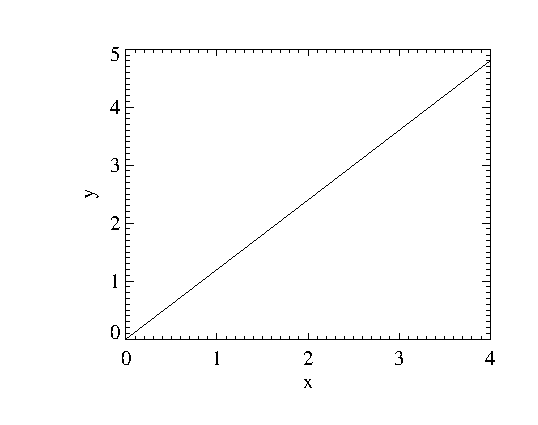
\includegraphics[width=3.75in]{simple.eps}
  \end{center}
  \caption{The caption of the figure.}
\label{fig:fig00}
\end{figure}%
\lipsum[12]

\subsubsection{Figure with psfrag replacement}

\lipsum[13].  Figure~\ref{fig:fig01} illustrates the use
of the psfrag package to place \LaTeX\ math in a graphic.%
\begin{figure}[tb]
  \psfrag{x}{$x$}
  \psfrag{y}{$y$}
  \begin{center}
   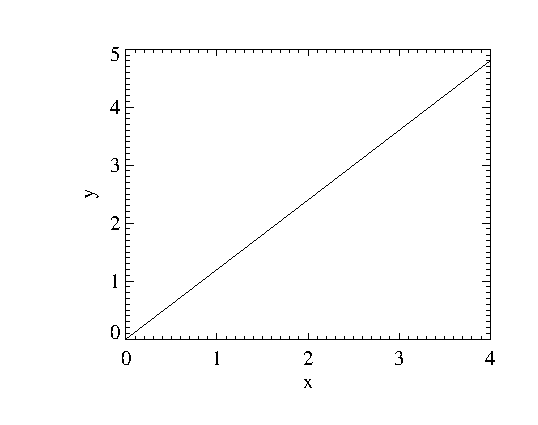
\includegraphics[width=3.75in]{simple.eps}
  \end{center}
  \caption[A figure caption which is extra long.]{A figure caption
    which is extra long. This long caption not only demonstratees that
    the required spacing in the list of figures is correct, but also
    the general practice of making the list of figures (or tables)
    entry the first sentence of the caption.}
\label{fig:fig01}
\end{figure}
\lipsum[14]. The filler content is followed by a second figure,
Figure~\ref{fig:fig02}.  %
\begin{figure}[tb]
  \psfrag{x}{$\hat{x}/L$}
  \psfrag{y}{$y$}
  \begin{center}
   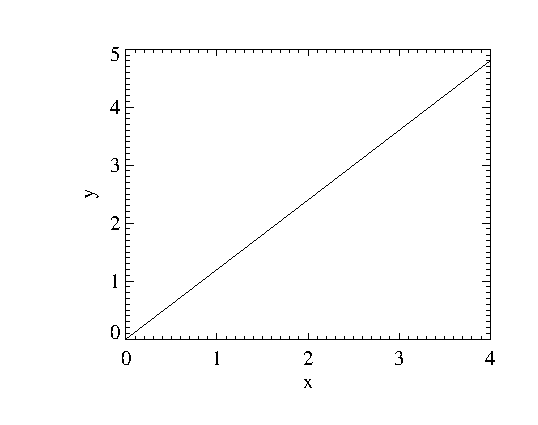
\includegraphics[width=3.75in]{simple.eps}
  \end{center}
  \caption{The figure caption made extra long so that the
    required spacing in the list of figures is evident.}
\label{fig:fig02}
\end{figure}
\lipsum[15]

\subsection{A Bit More Discussion}
\lipsum[16-19]


\endinput
%%
%% End of file `apxone.tex'.

\ThesisAppendixChapter{The Second Appendix Title}\input{apxtwo}
\end{ThesisAppendix}

%    \end{macrocode}
%
% \subsubsection{Back Matter - References and Vita}
%
%    \begin{macrocode}
 % ... references - comma separated list of bib files ...

\begin{ThesisBibliography}{REFERENCES}
%\newpage
 %\bibliographystyle{unsrtnat}
 %\bibliographystyle{ieeetr}
 %\bibliographystyle{plainnat}
\bibliographystyle{mstogs}
\singlespacing
\bibliography{add}
\end{ThesisBibliography}

 % ... vita ...

\begin{Vita}
\lipsum[4-5]
\end{Vita}

\end{document}
%</rpc>
%    \end{macrocode}
%
% \section{\LaTeX\ Template for Publication Thesis Option}
%
% \subsection{Using the Template}
%
% The steps in using the Publication Thesis Option template are the
% following
% \begin{enumerate}
% \item In each \verb|ppr.tex| file, change the class options
%   in the documentclass command to 
%   \verb|\documentclass[times,thesis]{journal}| where \emph{journal}
%   is the name of the journal the paper formatted for.  Once the class
%   options have been changed, re-make the file.  This should produce a 
%   postscript file with margins and pagination obeying the thesis
%   requirements.
% \item In each \verb|ppr.tex| file, add the following command
%   \verb|\setcounter{page}{x}| immediately following the 
%   \verb|\begin{document}| command, where \emph{x} is the starting page
%   number for the corresponding paper.  Now re-make each of the 
%   \verb|ppr.tex| files.  The result should be a thesis body with each of
%   the papers consituting it numbered consecutively.
% \item Edit the thesis.tex template by entering the correct paper names
%   and so on.  Compile the thesis template with the make command. Make
%   sure the pagination for the table of contents entries with the 
%   thesis body are correct.  Note that in the template, the setcounter
%   command will need to be issued with the correct page number corresponding
%   to each individual paper.
% \item Add (or uncomment) the \verb|\nofiles| command to the template
%   immediately preceding the \verb|\begin{document}| command.  This
%   command prevents \LaTeX\ from writing any changes to the 
%   \verb|.toc,.lof,.lot| files.  
% \item Add the entire contents from each \verb|ppr.lof| and \verb|ppr.lot|
%   to the corresponding template \verb|.lof| or \verb|.lot| file, at the 
%   appropriate place in these files.  Then recompile the 
%   template and be sure the the list of figures and list of tables entries
%   generated are correct.
% \item Now, go back to the individual \verb|ppr.tex| files and add
%   the \verb|\tableofcontents| command to each and re-make them.  Now
%   copy the contents of each of these individual \verb|.toc| files
%   to the \verb|.toc| file of the thesis template. Re-make the thesis.
% \item Print out the \verb|ppr.ps| files and the \verb|thesis.ps| files, 
%   put them in order and you have a complete thesis.
% \end{enumerate}
%
% \subsection{Additional Notes and Hints}
%
% \begin{itemize}
% \item If the bibliography in an individual entry needs to be edited
%   directly, edit the \verb|ppr.bbl| file but make sure not to re-run
%   the bibtex command because otherwise the changes will be overwritten.
% \item The \verb|nofiles| command cannot be used in the individual
%   \verb|ppr.tex| files since otherwise the nomenclature is not generated.
% \item In the thesis list of tables and list of illustrations, only an
%   abbreviated caption should appear.  This can be accomplished by editing
%   the \verb|.lof| and \verb|.lot| files.  Preferably, however, it can be
%   accomplished by using the following form of the caption command:
%   \verb|\caption[lst_entry]{heading}| where \verb|lst_entry| is the
%   abbreviated entry which is to appear in the list of figures or tables.
%   This can be the first sentence of the extended caption or an 
%   even more abbreviated version.
% \item The individual entries in the list of figures and tables for 
%   each paper must be set off by the following 
%   \verb|\noindent\mbox{PAPER 1\hfill}\nopagebreak|.  This should be 
%   added to the \verb|.lot| and \verb|.lof| files.
% \item The block of entries the \verb|.toc| must also be set off by a
%   command identical to the above.  In addition, this should be
%   preceded by \verb|\addvspace{\baselineskip}|.
% \item The list of figures and tables must also have single-spaced 
%   entries with doublespacing between the entries.  A way to 
%   accomplish this is to put the \verb|\singlespacing| command as the
%   second line of the \verb|.lot| and \verb|.lof| files and add,
%   immediately in front of each contentsline command, the following:
%   \verb|\addvspace{\baselineskip}|.  This same command will need to
%   be added in front of each of the above Paper x commands so that 
%   there is a blank line between the last entry of one paper and 
%   the line that says \verb|Paper x+1|.
% \item The entries in the table of contents must also be single spaced
%   for each entry and double-spaced between.  However, it is easier to
%   just let the table of contents be double-spaced and then put an
%   individual table of contents inside a singlespacing environment, if
%   it requires more than one line.
% \end{itemize}
%
% \subsection{Thesis Template}
%
% \subsubsection{Preamble}
%
% The preamble is ended by the \verb|\begin{document}| command.
% 
%    \begin{macrocode}
%<*pto>
 % -*- mode: LaTeX -*-
 % ... preamble ...
\documentclass[times,12pt,titlepage]{mstogs}

 % ... additions to ptotemplate ...
\usepackage[authoryear,sort]{natbib} % ... authoryear or numbers ...
\setlength{\bibhang}{0.5in}
\usepackage{docmute}
\usepackage{graphicx}
\usepackage{psfrag}
\usepackage{threeparttable}
\usepackage[noprefix]{nomencl}
\makenomenclature
\usepackage[sectionbib]{chapterbib}
\bibliographystyle{mstogs}

 % ... end of additions to ptotemplate ...

\doublespacing
\usepackage[nopar]{lipsum}

 % ... uncomment after editing toc, lof, lot ...

 %\nofiles

 % ... end preamble ...

\begin{document}

%    \end{macrocode}
%
% \subsubsection{Title Page}
%
%    \begin{macrocode}

 % ... specify: ms | phd ...

\begin{ThesisTitlePage}{phd}

\author{\MakeUppercase{Full Legal Name}}

\thesistitle{\MakeUppercase{The Title of My Work}}

\department{Mechanical Engineering}

 % ... thesis committee ...

\ThesisAdvisor{Ludwig Prandtl, Co-Advisor\\ Joe Miner, Co-Advisor}

\ThesisCommittee{%
Daniel Bernoulli\\ %
Leonard Euler\\ %
Pierre-Simon Laplace\\ %
Joseph Fourier}

 % ... Graduation date.  NOT your submission date! ...
\graddate{1685}       

\end{ThesisTitlePage}
%    \end{macrocode}
%
% \subsubsection{Copyright, Abstract and Acknowledgements}
%
%    \begin{macrocode}

 % ... copyright page - true|false ...

\copyrightyear{1685}
\ThesisCopyrightPage{true}

 % ... front matter - publication option - ms|phd...

\begin{ThesisPublicationOption}{phd}
  This \ThesisDissertationType\ consists of the following three
  articles which have been submitted for publication, or will be
  submitted for publication as follows:
\begin{quote}\begin{description}
\item Paper I: Pages x-xx have been submitted to ABC Journal.
\item Paper II: Pages x-xx are intended for submission to XYZ Journal.
\item Paper III: Pages x-xx have been accepted by 123 Journal.
\end{description}\end{quote}

\end{ThesisPublicationOption}

 % ... front matter - thesis abstract ...

\begin{ThesisAbstract}
\lipsum[1]
\end{ThesisAbstract}

 % ... front matter - acknowledgements ...

\begin{ThesisAcknowledgment}
\lipsum[2-3]
\end{ThesisAcknowledgment}

%    \end{macrocode}
%
% \subsubsection{Contents, Illustrations, Tables and Symbols}
%
%    \begin{macrocode}
 % ... toc, lof, and lot (list of symbols in respective papers) ...
\begin{ThesisFrontMatter}
\tableofcontents
\listoffigures
\listoftables
\end{ThesisFrontMatter}

%    \end{macrocode}
%
% \subsubsection{Thesis Body}
%
%    \begin{macrocode}
 % ... introduction chapter ...

\begin{ThesisBody}

\begin{ThesisOnlyChapters}{false}{false}
\ThesisBodyChapter{Introduction}\input{chpone}
\ThesisBodyChapter{Literature Review}\input{chptwo}
\end{ThesisOnlyChapters}

 % ... thesis publications ...

\begin{ThesisPublications}
\PaperManuscript{I}{FIRST PAPER WITH NO REFERENCES BUT REALLY LONG %
TITLE IN ORDER TO BE SURE IT IS CORRECTLY FORMATTED}\cbinput{pprone}
\PaperManuscript{II}{SECOND PAPER TITLE}\cbinput{pprtwo}
\PaperManuscript{III}{THIRD PAPER TITLE}\cbinput{pprthree}
\end{ThesisPublications}

 % ... conclusions chapter ...

\begin{ThesisOnlyChapters}{true}{true}
\ThesisBodyChapter{Unpublished Content}\input{chpthree}
\ThesisBodyChapter{Summary and Conclusions}%%
%% This is file `chpfive.tex',
%% generated with the docstrip utility.
%%
%% The original source files were:
%%
%% ths.dtx  (with options: `chapmin')
%% 
%% IMPORTANT NOTICE:
%% 
%% For the copyright see the source file.
%% 
%% Any modified versions of this file must be renamed
%% with new filenames distinct from chpfive.tex.
%% 
%% For distribution of the original source see the terms
%% for copying and modification in the file ths.dtx.
%% 
%% This generated file may be distributed as long as the
%% original source files, as listed above, are part of the
%% same distribution. (The sources need not necessarily be
%% in the same archive or directory.)


 %% ... sample chapter ...

\lipsum[6]

\section{A SECOND-LEVEL HEADING}
\lipsum[7-9]

\subsection{A Third-Level Heading}
\lipsum[10]
\subsubsection{A fourth-level heading with a very long and complicated title
to once again verify the formatting}
\lipsum[10-12]
\subsubsection{Another fourth-level heading}
\lipsum[10-12]

\subsection{Another Third-Level Heading but with a Very Long and
  Complicated Title to Verify the Formatting}
\lipsum[13-15]

\section{Discussion Using a Second-Level Heading
  Which is Really Long So That It Produces a Two-Line
  Toc Entry}
\lipsum[10-12]


\endinput
%%
%% End of file `chpfive.tex'.

\end{ThesisOnlyChapters}

\end{ThesisBody}

%    \end{macrocode}
%
% \subsubsection{Appendix}
%
%    \begin{macrocode}
 % ... appendix - specify number of appendix chapters ...

\begin{ThesisAppendix}{two}{false}{false}
\ThesisAppendixChapter{An Appendix Title}%%
%% This is file `apxone.tex',
%% generated with the docstrip utility.
%%
%% The original source files were:
%%
%% ths.dtx  (with options: `apxmin,addfig')
%% 
%% IMPORTANT NOTICE:
%% 
%% For the copyright see the source file.
%% 
%% Any modified versions of this file must be renamed
%% with new filenames distinct from apxone.tex.
%% 
%% For distribution of the original source see the terms
%% for copying and modification in the file ths.dtx.
%% 
%% This generated file may be distributed as long as the
%% original source files, as listed above, are part of the
%% same distribution. (The sources need not necessarily be
%% in the same archive or directory.)


 %% ... sample chapter ...

\section{A First-LEVEL Appendix HEADING}
\lipsum[7-9]

\subsection{A Second-Level Appendix Heading}
\lipsum[10]
\subsubsection{A Third-Level Appendix Heading with a Very Long and
  Complicated Title to Once Again Verify the Formatting}
\lipsum[10-12]
\subsubsection{Another Third-Level Appendix Heading}
\lipsum[10-12]
\paragraph{A fourth-level appendix heading with a long and complicated title
to once again verify the formatting}
\lipsum[13-15]

\subsection{Another Second-Level Appendix Heading but with a
Very Long and Complicated Title to Verify the Formatting}
\lipsum[13-15]

\section{Discussion Using a First-Level Appendix Heading
  Which is Really Long So That It Produces a Two-Line
  Toc Entry}
\lipsum[10-12]

\section{Content with Figures}
\lipsum[10]

\subsection{Floats with Figures}

\lipsum[12-13]

\subsubsection{Simple Figure with Label}

\lipsum[11]

Add a simple figure, Figure~\ref{fig:fig00}, to illustrate
an entry in the list of figures. %
\begin{figure}[tb]
  \begin{center}
   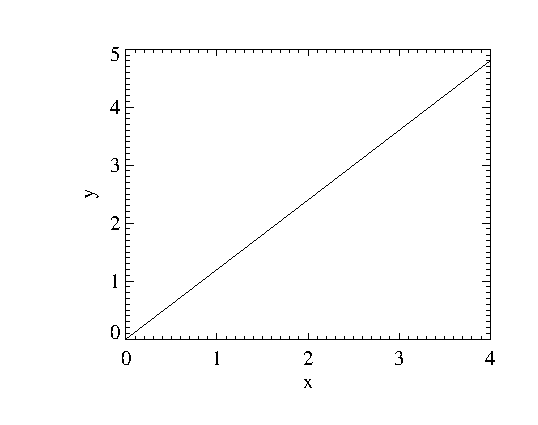
\includegraphics[width=3.75in]{simple.eps}
  \end{center}
  \caption{The caption of the figure.}
\label{fig:fig00}
\end{figure}%
\lipsum[12]

\subsubsection{Figure with psfrag replacement}

\lipsum[13].  Figure~\ref{fig:fig01} illustrates the use
of the psfrag package to place \LaTeX\ math in a graphic.%
\begin{figure}[tb]
  \psfrag{x}{$x$}
  \psfrag{y}{$y$}
  \begin{center}
   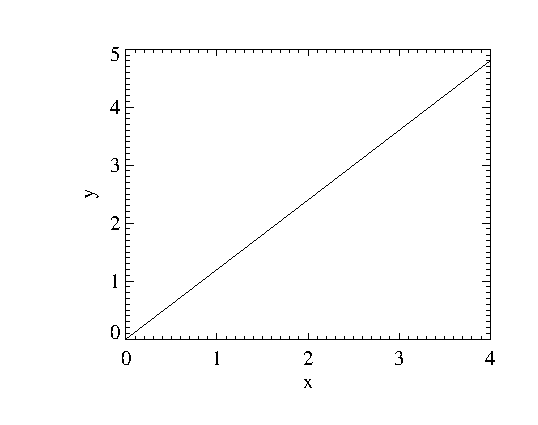
\includegraphics[width=3.75in]{simple.eps}
  \end{center}
  \caption[A figure caption which is extra long.]{A figure caption
    which is extra long. This long caption not only demonstratees that
    the required spacing in the list of figures is correct, but also
    the general practice of making the list of figures (or tables)
    entry the first sentence of the caption.}
\label{fig:fig01}
\end{figure}
\lipsum[14]. The filler content is followed by a second figure,
Figure~\ref{fig:fig02}.  %
\begin{figure}[tb]
  \psfrag{x}{$\hat{x}/L$}
  \psfrag{y}{$y$}
  \begin{center}
   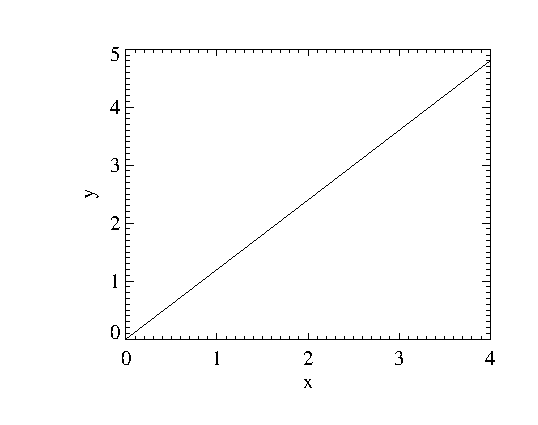
\includegraphics[width=3.75in]{simple.eps}
  \end{center}
  \caption{The figure caption made extra long so that the
    required spacing in the list of figures is evident.}
\label{fig:fig02}
\end{figure}
\lipsum[15]

\subsection{A Bit More Discussion}
\lipsum[16-19]


\endinput
%%
%% End of file `apxone.tex'.

\ThesisAppendixChapter{The Second Appendix Title}\input{apxtwo}
\end{ThesisAppendix}

%    \end{macrocode}
%
% \subsubsection{Back Matter - References and Vita}
%
%    \begin{macrocode}
 % ... references - comma separated list of bib files ...

\begin{ThesisBibliography}{REFERENCES}
\singlespacing
\bibliography{add}
\end{ThesisBibliography}

 % ... vita ...

\begin{Vita}
\lipsum[4-5]
\end{Vita}

 % ... end document ...

\end{document}
%</pto>
%    \end{macrocode}
%
% \section{\LaTeX\ Templates for Generic Chapter Content}
%
% \subsection{Minimal (text-only) Chapter Template}
%
%    \begin{macrocode}
%<*chapmin>

 %% ... sample chapter ...

\lipsum[6]

\section{A SECOND-LEVEL HEADING}
\lipsum[7-9]

\subsection{A Third-Level Heading}
\lipsum[10]
\subsubsection{A fourth-level heading with a very long and complicated title
to once again verify the formatting}
\lipsum[10-12]
\subsubsection{Another fourth-level heading}
\lipsum[10-12]

\subsection{Another Third-Level Heading but with a Very Long and
  Complicated Title to Verify the Formatting}
\lipsum[13-15]

\section{Discussion Using a Second-Level Heading 
  Which is Really Long So That It Produces a Two-Line 
  Toc Entry}
\lipsum[10-12]

%</chapmin>
%    \end{macrocode}
%
%
% \section{\LaTeX\ Templates for Generic Paper Content}
%
% \subsection{Minimal (text-only) Paper Template}
%
%    \begin{macrocode}
%<*pprmin>
 % ... preamble ...
\documentclass{article}
\usepackage[nopar]{lipsum}
\usepackage{graphicx}
\usepackage{threeparttable}

\newcommand{\ThesisPaperAuthor}[1]{\title{#1}}
\newenvironment{ThesisPaperAbstract}{\begin{abstract}}{\end{abstract}}
\newcommand{\ThesisPaperKeywords}[1]{\textbf{Keywords:} #1}

\begin{document}

 % ... title page ...

\ThesisPaperAuthor{%
 I.\ M.\ Author\\%
 Department of Mechanical \& Aerospace Engineering\\
 Missouri University of Science and Technology\\
 Rolla, Missouri 65409--0050\\
 Tel: 573--341--6622, Fax: 573--341--4115\\
 Email: imauthor@mst.edu%
}

 % ... abstract ...

\begin{ThesisPaperAbstract}
\lipsum[50-52]
\end{ThesisPaperAbstract}

 % ... keywords ...

\ThesisPaperKeywords{convection}

 % ... nomenclature - do not edit ...

%\frontglossary

 % ... introduction ...

\section{INTRODUCTION}

\lipsum[52-55]

\section{A First-Level Heading in a Paper Which is Really 
Long So That It Produces a Two-Line Toc Entry}
\lipsum[7-9]

\subsection{A SECOND-LEVEL HEADING IN A PAPER}
\lipsum[10]
\subsubsection{A Third-Level Heading in a Paper with a Very Long and
  Complicated Title to Once Again Verify the Formatting}
\lipsum[10-12]
\subsubsection{Another Third-Level Heading in a Paper}
\lipsum[10-12]
\paragraph{A fourth-level heading in a paper with a very long and complicated
  title to verify the formatting}
\lipsum[20]
\paragraph{Another fourth-level heading}
\lipsum[21]


\subsection{ANOTHER SECOND-LEVEL HEADING IN A PAPER WITH 
A VERY LONG AND COMPLICATED TITLE TO VERIFY THE FORMATTING}
\lipsum[13-15]

 % ... formulation ...

\section{Problem Formulation}%
  \label{sec:formulation}
\lipsum[56]

\subsection{GOVERNING EQUATIONS}

This is my simple equation
\begin{equation}
\delta_i = \sqrt{\nu t}
\end{equation}
where $\delta$ is the boundary layer thickness for Stokes' first
problem. %
\lipsum[57-60]

Figure~\ref{fig:fig01} %
\begin{figure}[t]
  \begin{center}
  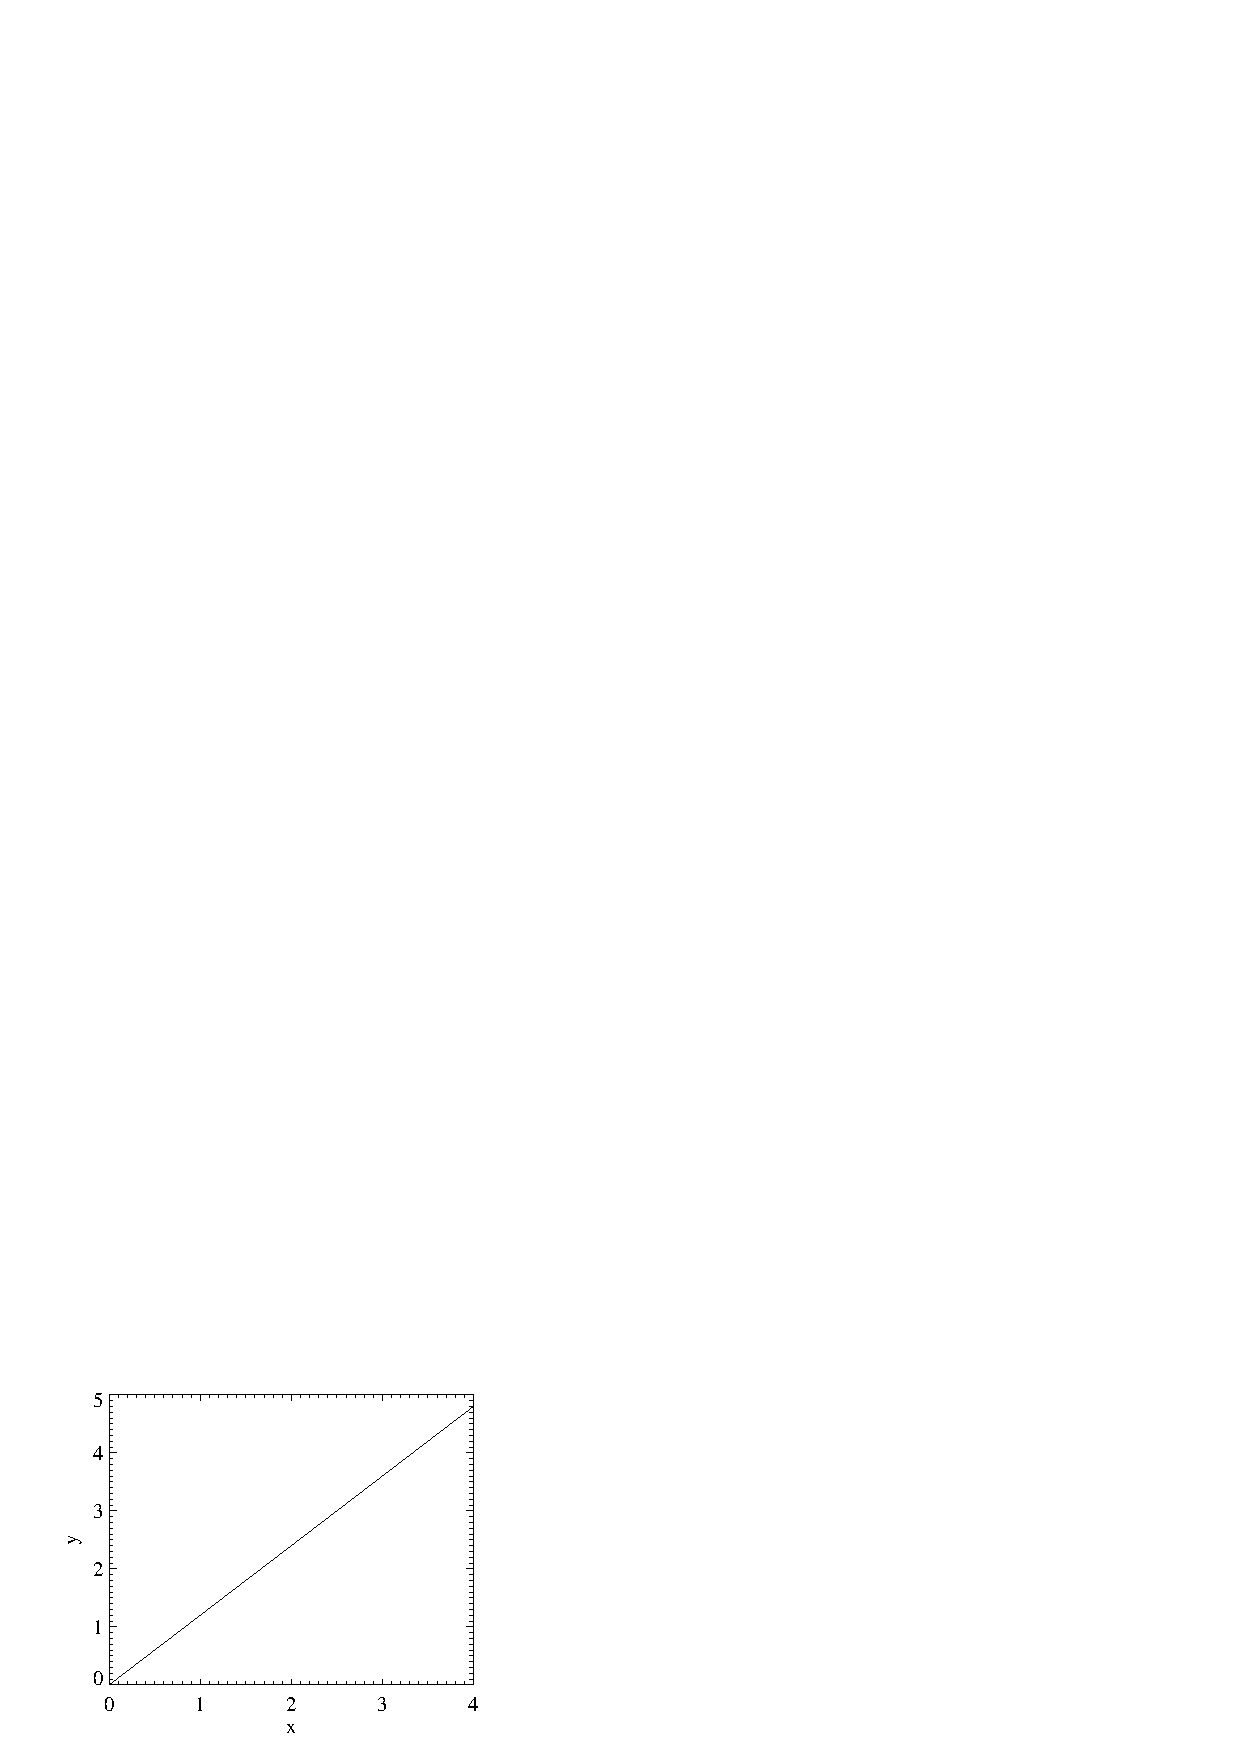
\includegraphics[width=3.75in]{simple.pdf}
  \end{center}
  \caption{The caption of the figure.}
\label{fig:fig01}
\end{figure}
illustrates the implementation of a very simple
figure. \lipsum[61-65].

Tables, such as Table~\ref{tbl:tbl01}, %
\begin{table}[t]
  \caption{The caption of the table should use capitalization
    consistent with that of the figures.}
  \label{tbl:tbl01}
  \begin{center}
  \begin{tabular}{c l l}
  \hline
  Example & Time & Cost \\
  \hline
  1 & 12.5 & \$1,000 \\
  2 & 24 & \$2,000 \\
  \hline
  \end{tabular}
  \end{center}
\end{table}
should appear in the order of their citation and should
generally appear at the top of the page in a final manuscript.
\lipsum[66-70]

 % ... results ...

\section{Results and Discussion} \label{sec:results}
\lipsum[71-80]

 % ... conclusions ...

\section{Conclusions}
\lipsum[81-85]

 % ... acknowledgments ...

\section*{Acknowledgements}      
\addcontentsline{toc}{section}{Acknowledgements}
\lipsum[2]

 % ... references - bib files ...

 %\bibliographystyle{plainnat}
 %\ThesisPaperReferences{add}

 % ... end ...

\end{document}

%</pprmin>
%    \end{macrocode}
%
% \subsection{Paper Template with Bibliography Citations}
%
%    \begin{macrocode}
%<*pprbib>
 % ... preamble ...
\documentclass{article}

\usepackage[nopar]{lipsum}
\usepackage{graphicx}
\usepackage{setspace}
\usepackage{threeparttable}
\usepackage{natbib}
\setlength{\bibhang}{0.5in}

\newcommand{\ThesisPaperAuthor}[1]{\title{#1}}
\newenvironment{ThesisPaperAbstract}{\begin{abstract}}{\end{abstract}}
\newcommand{\ThesisPaperKeywords}[1]{\textbf{Keywords:} #1}
\newenvironment{ThesisPaperBibliography}{}{}
\newcommand{\ThesisPaperReferences}[1]{\bibliography{#1}}

\begin{document}

 % ... title page ...

\ThesisPaperAuthor{%
 I.\ M.\ Author\\%
 Department of Mechanical \& Aerospace Engineering\\
 Missouri University of Science and Technology\\
 Rolla, Missouri 65409--0050\\
 Tel: 573--341--6622, Fax: 573--341--4115\\
 Email: imauthor@mst.edu%
}

%\date{}

%\maketitle

 % ... abstract ...

\begin{ThesisPaperAbstract}
\lipsum[52-55]
\end{ThesisPaperAbstract}

 % ... keywords ...

\ThesisPaperKeywords{convection}

 % ... introduction ...

\section{Introduction}

\lipsum[52-55]

 % ... formulation ...

\section{Problem Formulation}

\lipsum[56]
\subsection{GOVERNING EQUATIONS}

This is my simple equation
\begin{equation}
\delta_i = \sqrt{t/\mathrm{Pe}}
\end{equation}
where $\delta$ is the thermocline
thickness %
defined previously by \citep{bullwinkle.1990} and
\citet{winkle.1991}. \lipsum[57-60]

Figure~\ref{fig:fig01} %
\begin{figure}[t]
%  \psfrag{x}{\paxis{$x$}}
%  \psfrag{y}{\paxis{$y$}}
  \begin{center}
  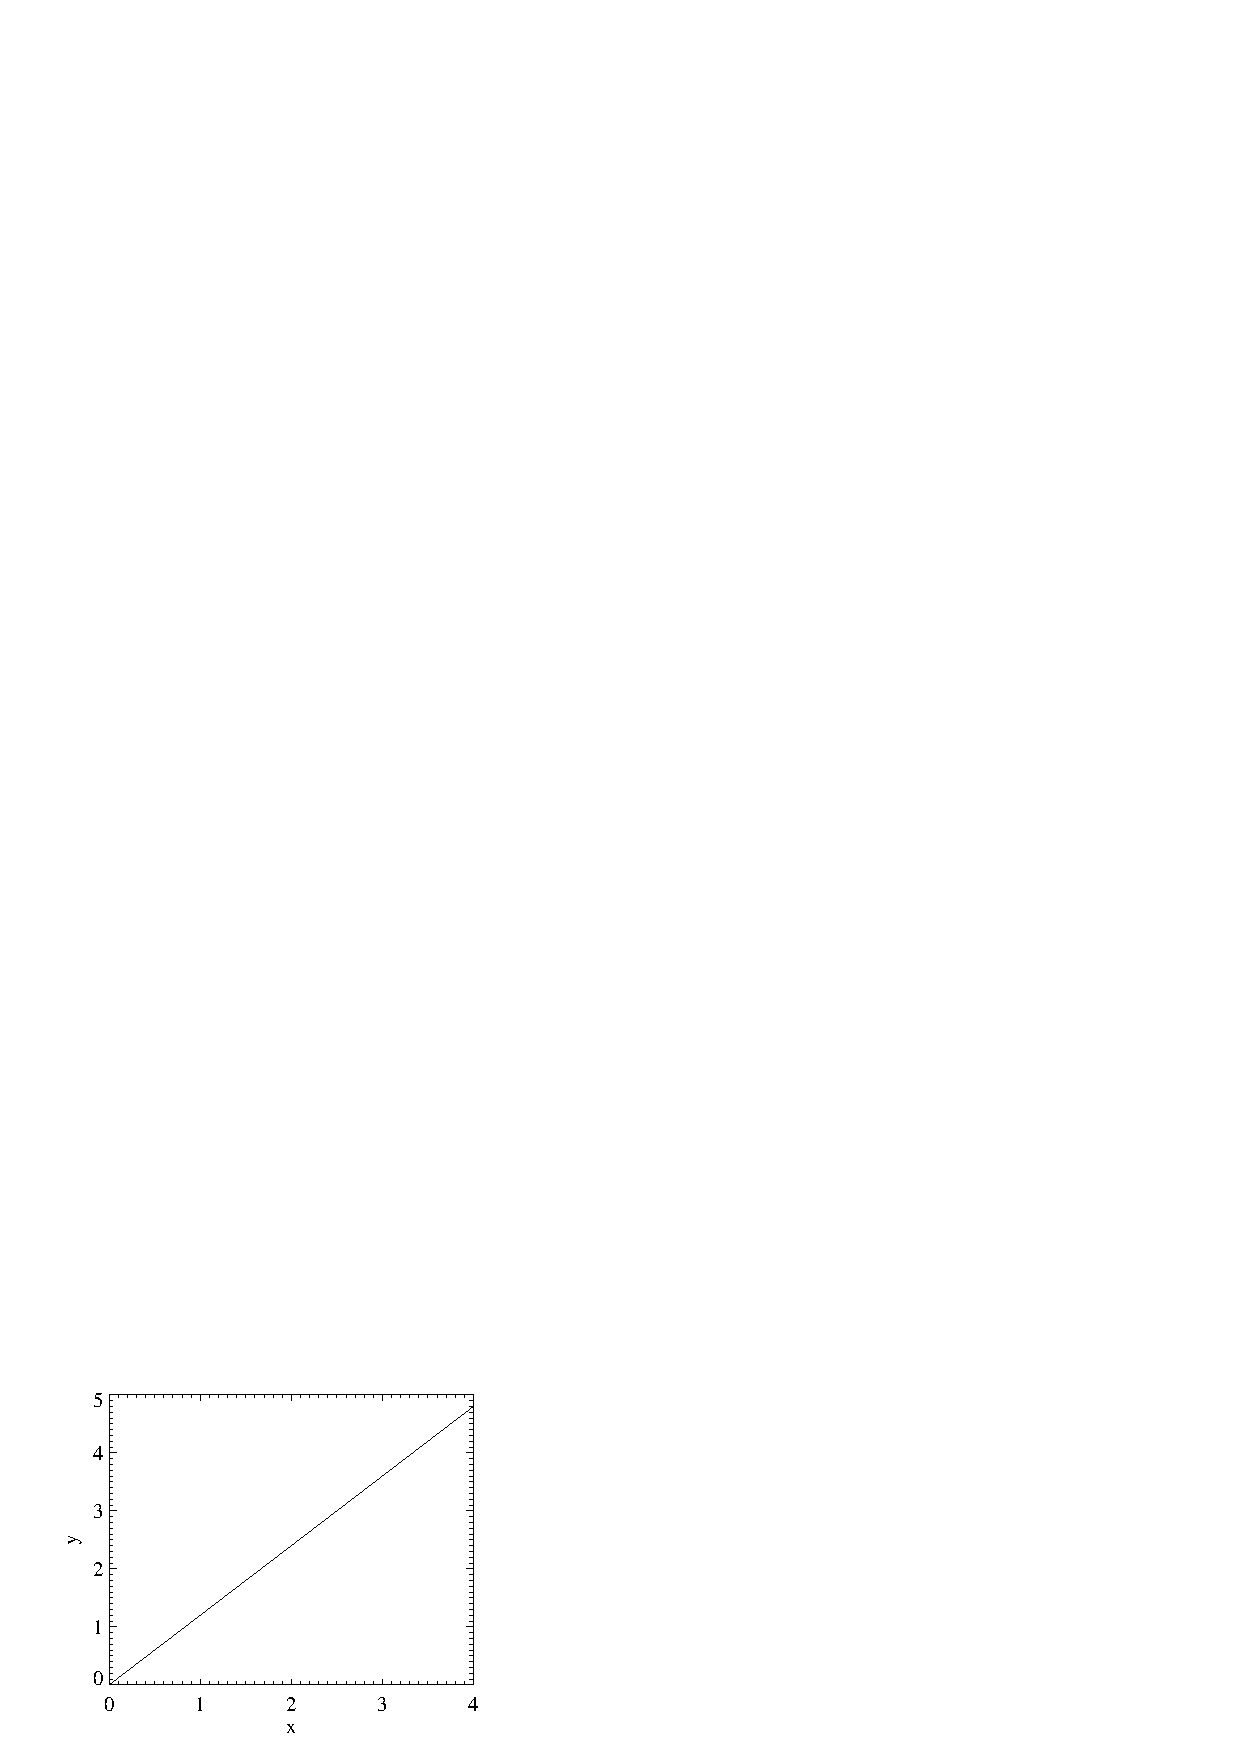
\includegraphics[width=3.75in]{simple.pdf}
  \end{center}
  \caption{The caption of the figure.}
\label{fig:fig01}
\end{figure}
illustrates the implementation of a very simple figure. \lipsum[61-65]

The inclusion of tables, such as Table~\ref{tbl:tbl01}, is just as
straigtforward. %
\begin{table}[t]
  \caption{The caption of the table should use capitalization
    consistent with that of the figures.}
  \label{tbl:tbl01}
  \begin{center}
  \begin{tabular}{c l l}
  \hline
  Example & Time & Cost \\
  \hline
  1 & 12.5 & \$1,000 \\
  2 & 24 & \$2,000 \\
  \hline
  \end{tabular}
  \end{center}
\end{table}
Tables should appear in the order of their citation and should
generally appear at the top of the page in a final manuscript. 
\lipsum[66-70]

 % ... results ...

\section{Results and Discussion} 
\lipsum[71-80]

 % ... conclusions ...

\section{Conclusions}
\lipsum[81-85]

 % ... acknowledgments ...

\section*{Acknowledgements}
\addcontentsline{toc}{section}{Acknowledgements}
\lipsum[86]

 % ... references - bib files ...

\begin{ThesisPaperBibliography}{REFERENCES}
\bibliographystyle{mstogs}
\singlespacing
\ThesisPaperReferences{add}
\end{ThesisPaperBibliography}

 % ... end ...

\end{document}

%</pprbib>
%    \end{macrocode}
%
% \subsection{Paper Template with All Content Elements}
%
%    \begin{macrocode}
%<*pprall>
 % ... preamble ...
\documentclass{article}

\usepackage[nopar]{lipsum}
\usepackage{graphicx}
\usepackage{threeparttable}
\usepackage{setspace}
\usepackage{natbib}
\setlength{\bibhang}{0.5in}
\usepackage[noprefix]{nomencl}
\makenomenclature

\newcommand{\ThesisPaperAuthor}[1]{\title{#1}}
\newenvironment{ThesisPaperAbstract}{\begin{abstract}}{\end{abstract}}
\newcommand{\ThesisPaperKeywords}[1]{\textbf{Keywords:} #1}
\newenvironment{ThesisPaperBibliography}{}{}
\newcommand{\ThesisPaperReferences}[1]{\bibliography{#1}}

\begin{document}

 % ... title page ...

%\title{%
%THE TITLE%
%\thanks{\LaTeX'd \today.}%
%}

\ThesisPaperAuthor{%
 I.\ M.\ Author\\%
 Department of Mechanical \& Aerospace Engineering\\
 Missouri University of Science and Technology\\
 Rolla, Missouri 65409--0050\\
 Tel: 573--341--6622, Fax: 573--341--4115\\
 Email: imauthor@mst.edu%
}

%\date{}

%\maketitle

 % ... abstract ...

\begin{ThesisPaperAbstract}
\lipsum[50]
\end{ThesisPaperAbstract}

 % ... keywords ...

\ThesisPaperKeywords{convection}

 % ... nomenclature - do not edit ...

%\frontglossary

 % ... introduction ...

\section{Introduction}
\lipsum[51-55]

 % ... formulation ...

\section{Problem Formulation}

\lipsum[56]

\subsection{GOVERNING EQUATIONS}

This is my simple equation
\begin{equation}
\delta_i = \sqrt{t/\mathrm{Pe}}
\end{equation}
where $\delta$ is the thermocline
thickness %
\nomenclature[at]{$t$}{time}%
\nomenclature[gd]{$\delta$}{thermocline thickness}%
\nomenclature[si]{$i$}{inlet}%
defined previously by \citep{bullwinkle.1990} and
\citet{winkle.1991}. \lipsum[57-60]

Figure~\ref{fig:fig01} %
\begin{figure}[t]
%  \psfrag{x}{\paxis{$x$}}
%  \psfrag{y}{\paxis{$y$}}
  \begin{center}
  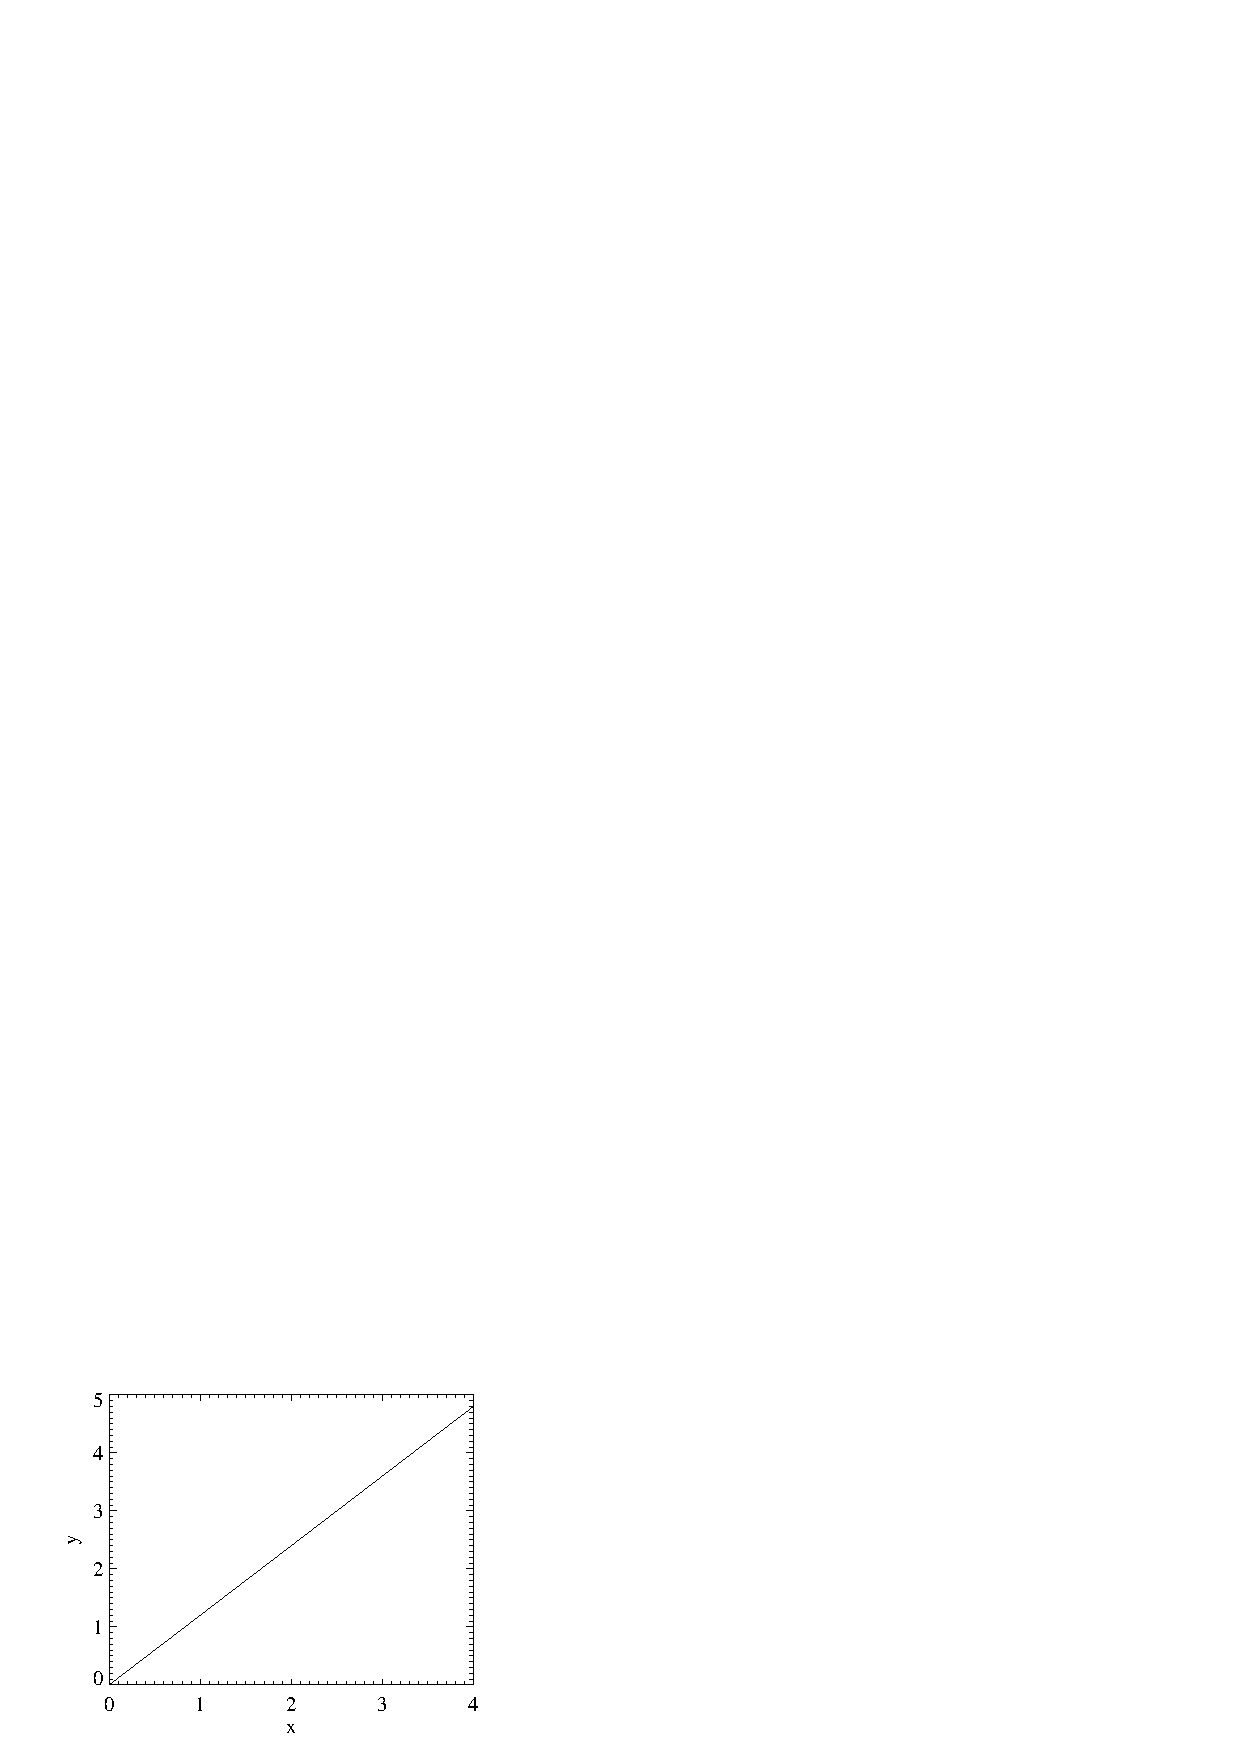
\includegraphics[width=3.75in]{simple.pdf}
  \end{center}
  \caption{The caption of the figure.}
\label{fig:fig01}
\end{figure}
\lipsum[61-65].

Tables, such as Tables~\ref{tbl:tbl01} and \ref{tbl:tbl02}, %
\begin{table}[t]
  \caption{The caption of the table uses sentence capitalization.}
  \label{tbl:tbl01}
  \begin{center}
  \begin{tabular}{c l l}
  \hline
  Example & Time & Cost \\
  \hline
  1 & 12.5 & \$1,000 \\
  2 & 24 & \$2,000 \\
  \hline
  \end{tabular}
  \end{center}
\end{table}
should appear in the order of their citation and should
\begin{table}[t]
\begin{threeparttable}
  \caption{The caption of the table uses sentence capitalization.}
  \label{tbl:tbl02}
  \begin{center}
\begin{tabular*}{\textwidth}{c l l} % or {tabular}
  \hline
  Example & Time\tnote{1} & Cost \\
  \hline
  1 & 12.5 & \$1,000 \\
  2 & 24 & \$2,000 \\
  \hline
\end{tabular*}
\begin{tablenotes}
  \item [1] The first note.
\end{tablenotes}
  \end{center}
\end{threeparttable}
\end{table}
generally appear at the top of the page in a final manuscript.
\lipsum[66-70]

 % ... results ...

\section{Results and Discussion}
\lipsum[71-80]

 % ... conclusions ...

\section{Conclusions}
\lipsum[81-85]

 % ... acknowledgments ...

\section*{Acknowledgements}
\addcontentsline{toc}{section}{Acknowledgements}
\lipsum[86]

 % ... nomenclature - do not edit ...

%\backglossary

 % ... references - bib files ...

\begin{ThesisPaperBibliography}{REFERENCES}
\bibliographystyle{mstogs}
\singlespacing
\ThesisPaperReferences{add}
\end{ThesisPaperBibliography}

 % ... end ...

 \end{document}

%</pprall>
%    \end{macrocode}
%
% \subsection{Minimal (text-only) Appendix  Template}
%
%    \begin{macrocode}
%<*apxmin>

 %% ... sample chapter ...

\section{A First-LEVEL Appendix HEADING}
\lipsum[7-9]

\subsection{A Second-Level Appendix Heading}
\lipsum[10]
\subsubsection{A Third-Level Appendix Heading with a Very Long and
  Complicated Title to Once Again Verify the Formatting}
\lipsum[10-12]
\subsubsection{Another Third-Level Appendix Heading}
\lipsum[10-12]
\paragraph{A fourth-level appendix heading with a long and complicated title
to once again verify the formatting}
\lipsum[13-15]

\subsection{Another Second-Level Appendix Heading but with a 
Very Long and Complicated Title to Verify the Formatting}
\lipsum[13-15]

\section{Discussion Using a First-Level Appendix Heading 
  Which is Really Long So That It Produces a Two-Line 
  Toc Entry}
\lipsum[10-12]

%</apxmin>
%    \end{macrocode}
%
% \subsection{Content with Figures}
%
%    \begin{macrocode}
%<*addfig>
\section{Content with Figures}
\lipsum[10]

\subsection{Floats with Figures}

\lipsum[12-13]

\subsubsection{Simple figure with label}

\lipsum[11]

Add a simple figure, Figure~\ref{fig:fig00}, to illustrate
an entry in the list of figures. %
\begin{figure}[tb]
  \begin{center}
   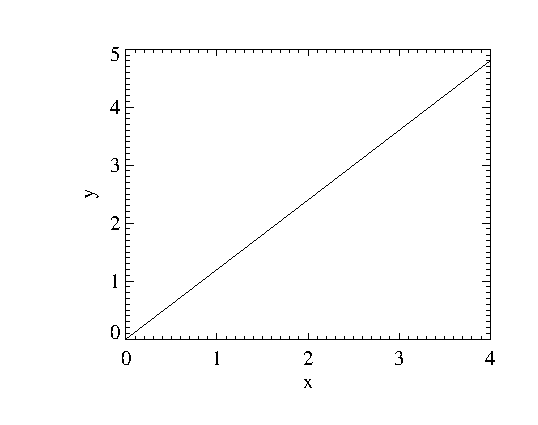
\includegraphics[width=3.75in]{simple.eps}
  \end{center}
  \caption{The caption of the figure.}
\label{fig:fig00}
\end{figure}%
\lipsum[12]

\subsubsection{Figure with psfrag replacement}

\lipsum[13].  Figure~\ref{fig:fig01} illustrates the use
of the psfrag package to place \LaTeX\ math in a graphic.%
\begin{figure}[tb]
  \psfrag{x}{$x$}
  \psfrag{y}{$y$}
  \begin{center}
   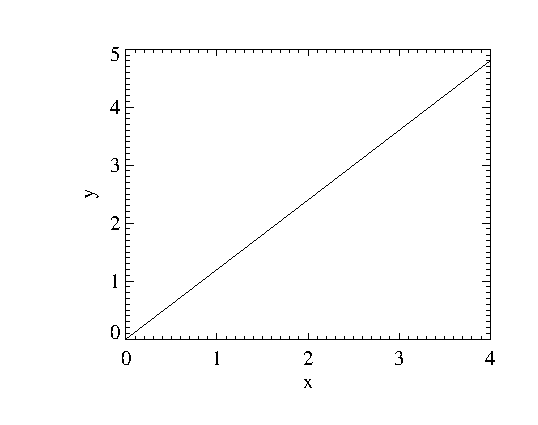
\includegraphics[width=3.75in]{simple.eps}
  \end{center}
  \caption[A figure caption which is extra long.]{A figure caption
    which is extra long. This long caption not only demonstratees that
    the required spacing in the list of figures is correct, but also
    the general practice of making the list of figures (or tables)
    entry the first sentence of the caption.}
\label{fig:fig01}
\end{figure}
\lipsum[14]. The filler content is followed by a second figure,
Figure~\ref{fig:fig02}.  %
\begin{figure}[tb]
  \psfrag{x}{$\hat{x}/L$}
  \psfrag{y}{$y$}
  \begin{center}
   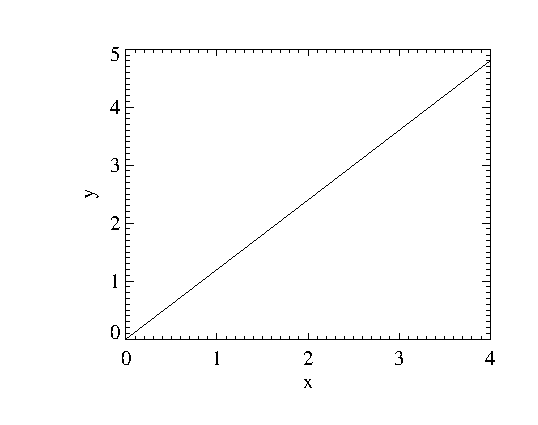
\includegraphics[width=3.75in]{simple.eps}
  \end{center}
  \caption{The figure caption made extra long so that the
    required spacing in the list of figures is evident.}
\label{fig:fig02}
\end{figure}
\lipsum[15]

\subsection{A Bit More Discussion}
\lipsum[16-19]

%</addfig>
%    \end{macrocode}
%
% \subsection{Content with Tables}
%
%    \begin{macrocode}
%<*addtbl>
\section{Content with Sample Tables}

\lipsum[15]

\subsection{Floats with Tables}

\lipsum[16]

\subsubsection{Simple table}

Finally the tables, Table~\ref{tbl:tbl01} illustrates the syntax of a
basic table. %
\begin{table}[tb]
  \caption{The capitalization of the table should match that of figures.}
  \label{tbl:tbl01}
  \begin{center}
  \begin{tabular}{c l l}
  \hline
  Example & Time & Cost \\
  \hline
  1 & 12.5 & \$1,000 \\
  2 & 24 & \$2,000 \\
  \hline
  \end{tabular}
  \end{center}
\end{table}
\lipsum[16-18]

\subsubsection{Three-part table example}

Table~\ref{tbl:tbl02}, which illustrates the syntax of a three-part
table which includes table notes in addition to a caption and table
body.
\begin{table}[tb]
\begin{threeparttable}
  \caption{The caption of the three-part table.}
  \label{tbl:tbl02}
  \begin{center}
\begin{tabular*}{\textwidth}{c l l} % or {tabular}
  \hline
  Example & Time\tnote{1} & Cost \\
  \hline
  1 & 12.5 & \$1,000 \\
  2 & 24 & \$2,000 \\
  \hline
\end{tabular*}
\begin{tablenotes}
  \item [1] The first note.
\end{tablenotes}
  \end{center}
\end{threeparttable}
\end{table}
\lipsum[19-21]

\subsection{One More Thing}
\lipsum[22-25]
%</addtbl>
%    \end{macrocode}
%
% \subsection{Content with \texttt{natbib} Citations}
%
%    \begin{macrocode}
%<*addbib>

\section{Content with \texttt{natbib} Citations}

This had been discussed previously by \citep{bullwinkle.1990} and
\citet{winkle.1991}. \lipsum[22-25]

%</addbib>
%    \end{macrocode}
%
% \subsection{Content with \texttt{nomencl} Entries} 
%
%    \begin{macrocode}
%<*addglo>

\section{Content with \texttt{nomencl} Entries} 

Finally, we add a simple equation to illustrate the use of the nomencl
 package for automatic generation of a list of symbols.
\begin{equation}
\delta_i = \sqrt{t/\mathrm{Pe}}
\end{equation}
where $\delta$ is the layer
thickness %
\nomenclature[at]{$t$}{time}%
\nomenclature[gd]{$\delta$}{layer thickness}%
\nomenclature[si]{$i$}{inlet}%
as defined previously. \lipsum[26-30]
%</addglo>
%    \end{macrocode}
%
%

\endinput       

